
\section{Evaluation}
All experiments were run on Amazon EC2 using the p3.16xlarge instances.  Each instance has 8 Tesla V100 GPUs with 25Gbps Eternet bandwidth.  When possible, we launched instances in a placement group for faster inter-node network connection.  We conducted the following experiments:

\begin{enumerate}
    \item An end-to-end macrobencmark measuring training througput, for all three systems, utilizing up to 16 distinct instances (Figure~\ref{fig:sgd}).
    \item A microbenchmark that investigates a key limitation of our implementation: that using 8 GPUs per node yields worse scaling than using 4 GPUs per node, keeping the total number of GPUs constant (Figure~\ref{fig:8-vs-4-gpu}).
    \item A microbenchmark that investigates the best all-reduce strategies to use, within a node (Figure~\ref{fig:intra-node-allreduce-strategy}).
\end{enumerate}

% \subsection{Single-Node Multi GPU SGD}
% Here we discuss some findings on Multi-GPU
% \subsection{Charts}

\subsection{Macrobenchmark}
Figure~\ref{fig:sgd} shows the training throughput on ResNet-101 for three systems, Horovod, Distributed TensorFlow, and Ray (codenamed ``Halo'' in the graph).  In summary, our implementation in Ray is able to match Horovod and comes within 10\% of Distributed TensorFlow.  This result validates our hypothesis that the higher-level actor/task abstractions are able to match the SPMD/message-passing abstractions.

{\bf Weak Scaling.}  We note that the weak scaling factors, with 4 GPUs as baseline and with $2\times$ resource scaling at each step, are 1.9$\times$,1.9$\times$,3.7$\times$,7.3$\times$ for Horovod;
1.8$\times$,2.7$\times$,5.0$\times$,8.5$\times$ for Distributed TensorFlow;
and
1.8$\times$,2.2$\times$,4.1$\times$,7.3$\times$ for Ray.  Clearly, even the observed maximum 8.5$\times$ scaling  is far from ideal since $16\times$ as many GPUs are used; we surmise this is the exact reason that motivated several projects that investigate fast inter-GPUs interconnect, such as  NVIDIA's NVLink.

\begin{figure}
    \centering
    % 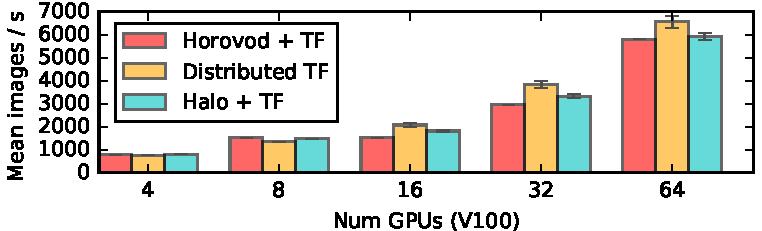
\includegraphics[width=3.1in,keepaspectratio]{fig/sgd_plot.pdf}
    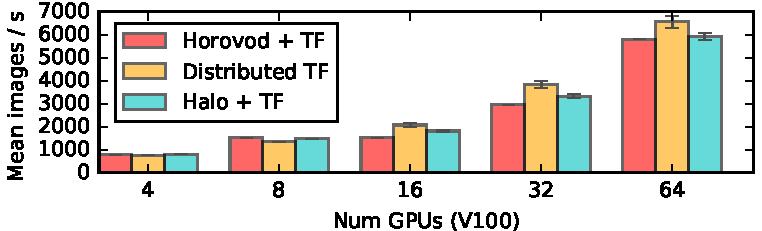
\includegraphics{fig/sgd_plot.pdf}
    \caption{
    \small{
        Images per second reached when distributing the training of a
        ResNet-101 TensorFlow model (from the official TF benchmark).
        %The \System{} implementation matches the performance of Horovod and
        %is within 10\% of distributed TensorFlow.
        All experiments were run on p3.16xl instances connected by 25Gbps Ethernet, and
        workers allocated 4 GPUs per node as done in Horovod~\cite{horovod}.
        We note some measurement deviations from previously reported, likely
        due to hardware differences and
        recent TensorFlow performance improvements. We used
        OpenMPI 3.0, TF 1.8, and NCCL2 for all runs.
    }
    }
    \label{fig:sgd}
\end{figure}

\subsection{Scaling Anomalies}
Through our investigation we discovered two interesting scaling anomalies, as
shown in Figure~\ref{fig:8-vs-4-gpu}.

First, one of the compared systems, Horovod, yields a lower throughput when 16
GPUs (2 nodes) are used, compared to 8 GPUs (1 node).  This suggests that
Horovod's cross-machine communication overhead is so large that it dwarfs the
benefits of using twice as many processors.

Second, for our Ray implementation, using 8 GPUs per node (red bars) scales
noticeably worse than using 4 GPUs per node (blue bars), while fixing the total
number of GPUs fixed.  The former cases make use of less number of machines, so
cross-node communication should actually be faster than the latter cases.  For
this reason, we hypothesize that the bottleneck stems from the intra-node
codepath.

\begin{figure}
    \centering
    % 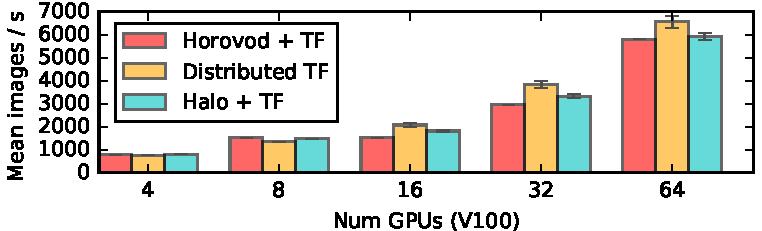
\includegraphics[width=3.1in,keepaspectratio]{fig/sgd_plot.pdf}
    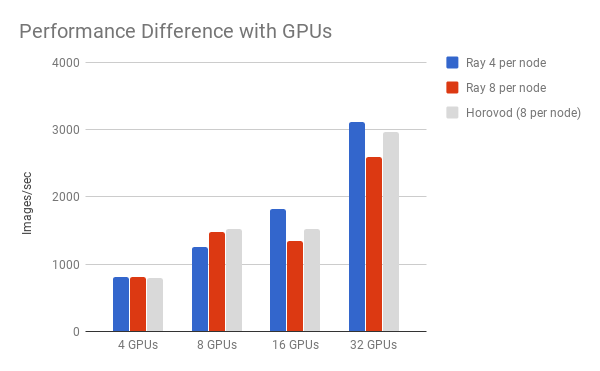
\includegraphics[width=3.1in,keepaspectratio]{fig/4to8.png}
    \caption{
    \small{
        Performance differences for using 4 GPUs per node vs 8 GPUs per node. In all cases, we use the same hardware (p3.16xlarge). However, we see there are performance differences going from 4 GPUs to 8 GPUs when comparing the number of GPUs per node. We provide Horovod performance for reference.
    }
    }
    \label{fig:8-vs-4-gpu}
\end{figure}

\begin{figure}
    \centering
    % 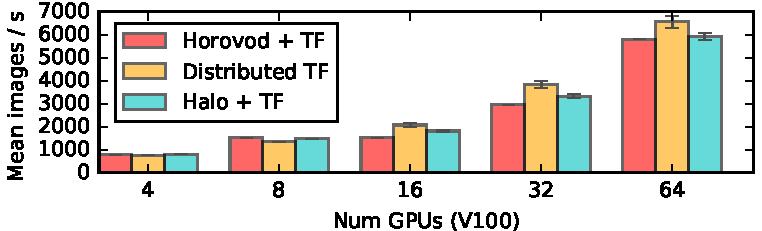
\includegraphics[width=3.1in,keepaspectratio]{fig/sgd_plot.pdf}
    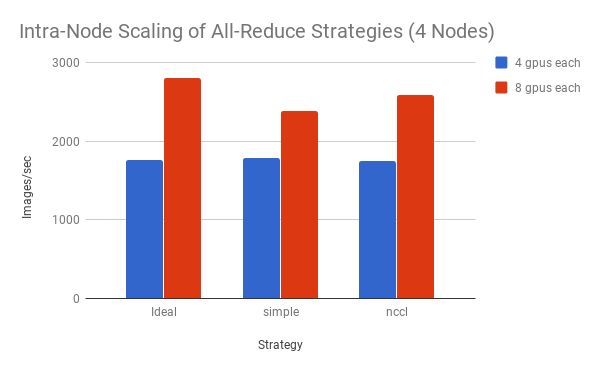
\includegraphics[width=3.1in,keepaspectratio]{fig/intranode.png}
    \caption{
    \small{
        Changing the all reduce strategy among GPUs within a node, and running a synchronous parameter server strategy between nodes. Ideal is generated by taking the gradient of the a single GPU, bypassing any communication overhead between GPUs on a single machine. "Simple" performance simply takes an average across all of the GPUs {\color{red} TODO: FIX THIS.}. "NCCL" performance uses the NCCL communication primitives to perform an all-reduce across the GPUs. We see that even though NCCL performance is better at 8 GPUs than "Simple", both provide sublinear scaling when doubling the number of GPUs per machine.
    }
    }
    \label{fig:intra-node-allreduce-strategy}
\end{figure}
